\documentclass[main.tex]{subfiles}

\begin{document}

\section*{\Huge\textcolor{mantis}{Neural Networks \& Backpropagation}}
\addcontentsline{toc}{section}{Neural Networks \& Backpropagation}
\vspace{0.5cm}

\needspace{0.33\textheight}
\section{The Perceptron Algorithm}

Binary classification is the task of classifying data into two categories. Given data with labels, we seek to learn the classifier. Inspired by neurons in the brain, the Perceptron algorithm learns a binary classifier from labeled data.

\subsection{Problem Setting}

Consider labeled data $(x, l(x))$, where $x \in X \subset \mathbb{R}^n$, $l(x) \in \{1, -1\}$. Each data point is labeled as:
$$l(x) = \text{sign}(\langle w^*, x \rangle) = \text{sign}\left(\sum_{i=1}^{n} w_i^* x_i\right)$$

Here $w^* \in \mathbb{R}^n$ is the unknown normal vector to a separating hyperplane. We assume that $\|w^*\| = 1$ and $\|x\| \leq 1$ for all data points.

\begin{definition}[Margin]
The \textbf{margin} for $w^*$ is defined as:
$$\gamma := \min_{x \in D} |\langle w^*, x \rangle|$$
\end{definition}

This implies that for any $x$ with label $l(x) = 1$, we have $\langle w^*, x \rangle \geq \gamma$; for any $x$ with label $l(x) = -1$, we have $\langle w^*, x \rangle \leq -\gamma$.

%%need to adjust this tikz figure, gamma is not shown properly... will claude this one :)

\begin{center}
\begin{tikzpicture}[scale=1.1]
    % Main separating hyperplane (solid black) - line y = 0.5x
    \draw[thick, black] (-3,-1.5) -- (3,1.5);
    
    % Margin lines (dashed, parallel to separator)
    \draw[dashed, black] (-3,-0.5) -- (3,2.5);  % upper margin: y = 0.5x + 1
    \draw[dashed, black] (-3,-2.5) -- (3,0.5);  % lower margin: y = 0.5x - 1
    
    % Normal vector w* (perpendicular to separator, pointing to + class)
    % Perpendicular direction to slope 0.5 is (-1, 2) normalized
    \draw[->, thick, black] (0,0) -- (-0.8,1.6);
    \node[black] at (-0.5,1.8) {$w^*$};
    
    % Gamma annotations - PERPENDICULAR to separator
    % From point (1, 0.5) on separator to upper margin at (0.6, 1.3)
    \draw[<->, thick, green!50!black] (1,0.5) -- (0.6,1.3);
    \node[green!50!black] at (1.1,1.0) {$\gamma$};
    % From point (1, 0.5) on separator to lower margin at (1.4, -0.3)
    \draw[<->, thick, green!50!black] (1,0.5) -- (1.4,-0.3);
    \node[green!50!black] at (1.5,0.2) {$\gamma$};
    
    % Positive points (+) - blue, above upper margin
    \node[blue, font=\bfseries\large] at (-2,1.5) {$+$};
    \node[blue, font=\bfseries\large] at (-1,2.2) {$+$};
    \node[blue, font=\bfseries\large] at (0,2.5) {$+$};
    \node[blue, font=\bfseries\large] at (1,2.8) {$+$};
    \node[blue, font=\bfseries\large] at (0.6,1.3) {$+$};  % support vector on margin
    \node[blue, font=\bfseries\large] at (1.5,2.3) {$+$};
    \node[blue, font=\bfseries\large] at (-1.5,2.0) {$+$};
    \node[blue, font=\bfseries\large] at (2,2.9) {$+$};
    
    % Negative points (-) - orange, below lower margin
    \node[orange, font=\bfseries\large] at (2,-0.5) {$-$};
    \node[orange, font=\bfseries\large] at (1,-0.8) {$-$};
    \node[orange, font=\bfseries\large] at (1.4,-0.3) {$-$};  % support vector on margin
    \node[orange, font=\bfseries\large] at (-1,-1.5) {$-$};
    \node[orange, font=\bfseries\large] at (1.5,-1.2) {$-$};
    \node[orange, font=\bfseries\large] at (2.5,-0.8) {$-$};
    \node[orange, font=\bfseries\large] at (0.5,-1.8) {$-$};
    \node[orange, font=\bfseries\large] at (-0.5,-2.0) {$-$};
\end{tikzpicture}
\end{center}

\subsection{Geometric Interpretation of the Weight Vector}

The weight vector $w$ has a fundamental geometric meaning: it is \textbf{orthogonal to the separating hyperplane}.

\begin{proposition}
The weight vector $w$ is normal to the decision boundary $H = \{x : \langle w, x \rangle = 0\}$.
\end{proposition}

\begin{proof}
Let $x_1, x_2 \in H$ be any two points on the hyperplane. Then:
$$\langle w, x_1 \rangle = 0 \quad \text{and} \quad \langle w, x_2 \rangle = 0$$

Subtracting: $\langle w, x_1 - x_2 \rangle = 0$. Since $x_1 - x_2$ is an arbitrary vector lying in $H$, we conclude that $w \perp H$.
\end{proof}

\begin{proposition}[Signed Distance to Hyperplane]
The signed distance from a point $x$ to the hyperplane $H = \{z : \langle w, z \rangle = 0\}$ is:
$$\text{dist}(x, H) = \frac{\langle w, x \rangle}{\|w\|}$$
\end{proposition}

\begin{proof}
Let $x_0 \in H$ be any point on the hyperplane, so $\langle w, x_0 \rangle = 0$. The signed distance is the projection of $(x - x_0)$ onto the unit normal $\frac{w}{\|w\|}$:
\begin{align}
\text{dist}(x, H) &= \langle x - x_0, \frac{w}{\|w\|} \rangle \\[6pt]
&= \frac{\langle x, w \rangle - \langle x_0, w \rangle}{\|w\|} \\[6pt]
&= \frac{\langle w, x \rangle - 0}{\|w\|} = \frac{\langle w, x \rangle}{\|w\|}
\end{align}
\end{proof}

\subsection{The Geometry of Weight Updates}

When we update the weight vector $w \leftarrow w + l(x)x$, we are \textbf{tilting the hyperplane} toward the misclassified point.

\begin{proposition}[Update Improves Classification]
If $(x, l(x))$ is misclassified under $w$, then after the update $\tilde{w} = w + l(x)x$:
$$l(x) \langle \tilde{w}, x \rangle > l(x) \langle w, x \rangle$$
\end{proposition}

\begin{proof}
We compute:
\begin{align}
l(x) \langle \tilde{w}, x \rangle &= l(x) \langle w + l(x)x, x \rangle \\[6pt]
&= l(x) \langle w, x \rangle + l(x)^2 \|x\|^2 \\[6pt]
&= l(x) \langle w, x \rangle + \|x\|^2
\end{align}

Since $\|x\|^2 > 0$, the improvement is strictly positive.
\end{proof}

\needspace{0.33\textheight}
\section{The Perceptron Algorithm}

\begin{algorithm}[Perceptron]
\textbf{Input:} Labeled data $\{(x_i, l(x_i))\}_{i=1}^n$ with $l(x_i) \in \{-1, +1\}$

\textbf{Output:} Weight vector $w$

\begin{enumerate}
    \item Start with $w = 0$
    \item \textbf{for each} input $x$ \textbf{do}
    \begin{enumerate}
        \item Predict $\text{sign}(\langle w, x \rangle)$
        \item On a mistake, set $w \leftarrow w + l(x)x$
    \end{enumerate}
    \item \textbf{end for}
\end{enumerate}
\end{algorithm}

\needspace{0.33\textheight}
\section{Convergence Analysis}

\begin{theorem}[Perceptron Convergence Bound]
The number of mistakes made by the Perceptron Algorithm on any input sequence is at most $1/\gamma^2$.
\end{theorem}

\begin{proof}
Consider the potential function $\frac{\langle w, w^* \rangle}{\|w\|}$, starting at $0$. Whenever the algorithm makes a mistake, we update $\tilde{w} := w + l(x)x$. We analyze the numerator and denominator separately.

\textbf{Step 1: Lower bound on the numerator.}

\begin{align}
\langle \tilde{w}, w^* \rangle &= \langle w + l(x)x, w^* \rangle \\[6pt]
&= \langle w, w^* \rangle + l(x)\langle x, w^* \rangle \\[6pt]
&\geq \langle w, w^* \rangle + \gamma
\end{align}

The last inequality follows from the definition of margin $\gamma$: since $l(x) = \text{sign}(\langle w^*, x \rangle)$, we have $l(x)\langle x, w^* \rangle = |\langle x, w^* \rangle| \geq \gamma$.

\textbf{Step 2: Upper bound on the denominator.}

\begin{align}
\|\tilde{w}\|^2 &= \langle \tilde{w}, \tilde{w} \rangle \\[6pt]
&= \langle w + l(x)x, w + l(x)x \rangle \\[6pt]
&= \langle w, w \rangle + \langle x, x \rangle + 2l(x)\langle w, x \rangle
\end{align}

Since $x$ is incorrectly predicted by $w$, we know $l(x) \neq \text{sign}(\langle w, x \rangle)$. This implies that $l(x)\langle w, x \rangle \leq 0$. Also, we assume that $\|x\| \leq 1$. Therefore:
$$\|\tilde{w}\|^2 \leq \langle w, w \rangle + \langle x, x \rangle \leq \|w\|^2 + 1$$

\textbf{Step 3: Induction after $T$ mistakes.}

By induction, after $T$ mistakes:
\begin{itemize}
    \item Numerator: $\langle \tilde{w}, w^* \rangle \geq \gamma T$
    \item Denominator: $\|\tilde{w}\| \leq \sqrt{T}$
\end{itemize}

\textbf{Step 4: Combining via Cauchy-Schwarz.}

By the Cauchy-Schwarz inequality:
$$|\langle \tilde{w}, w^* \rangle| \leq \|\tilde{w}\| \|w^*\| = \|\tilde{w}\|$$

since $\|w^*\| = 1$. This implies that $\frac{\langle \tilde{w}, w^* \rangle}{\|\tilde{w}\|} \leq 1$ at all time steps. Therefore:
$$1 \geq \frac{\langle \tilde{w}, w^* \rangle}{\|\tilde{w}\|} \geq \frac{\gamma T}{\sqrt{T}} = \gamma\sqrt{T}$$

It follows that:
$$\boxed{T \leq \frac{1}{\gamma^2}}$$
\end{proof}

\needspace{0.33\textheight}
\section{Lower Bound for the Perceptron Algorithm}

Theorem 3.1 shows that the number of mistakes is bounded by $1/\gamma^2$. However, when the margin is tiny, for instance $\gamma \sim 1/2^n$, the number of mistakes can be as large as $2^{O(n)}$, which is not polynomial with respect to the input dimension $n$.

We construct a dataset and show that for any given order, the Perceptron algorithm needs to see at least $2^{O(n)}$ examples before reaching the truth.

\subsection{The Hard Instance Construction}

For each data point $x^{(i)} \in \mathbb{R}^n$ with $i$ non-zero entries, we construct:

\begin{center}
\begin{tabular}{ccc}
\hline
& $x$ & $l(x)$ \\
\hline
$x^{(1)}$ & $(1, 0, 0, 0, \cdots, 0)$ & $+1$ \\
$x^{(2)}$ & $(1, -1, 0, 0, \cdots, 0)$ & $-1$ \\
$x^{(3)}$ & $(-1, -1, 1, 0, \cdots, 0)$ & $+1$ \\
$x^{(4)}$ & $(1, 1, 1, -1, 0, \cdots, 0)$ & $-1$ \\
$\vdots$ & $\vdots$ & $\vdots$ \\
$x^{(i)}$ & $((-1)^i, \cdots, (-1)^i, (-1)^{i+1}, 0, \cdots, 0)$ & $(-1)^{i+1}$ \\
\hline
\end{tabular}
\end{center}

\begin{lemma}
For a unit vector $w^* \in \mathbb{R}^n$ that classifies the data above correctly, its $i$-th coordinate satisfies $w^*_i \geq 2^{i-1}$.
\end{lemma}

\begin{proof}
By rescaling $w^*$, we can assume WLOG that the margin is $\gamma = 1$.

\textbf{Base case:} Since $l(x^{(1)}) = 1$, we have $\langle w^*, x^{(1)} \rangle \geq 1$. This gives $w^*_1 \geq 1 = 2^0$.

\textbf{Inductive step:} Similarly, we have $\langle w^*, x^{(2)} \rangle \leq -1$, which gives $w^*_1 - w^*_2 \leq -1$, and thus $w^*_2 \geq w^*_1 + 1$.

More generally, for odd $i$:
$$\langle w^*, x^{(i)} \rangle = -\sum_{j=1}^{i-1} w^*_j + w^*_i \geq 1 \quad \Rightarrow \quad w^*_i \geq \sum_{j=1}^{i-1} w^*_j + 1$$

For even $i$:
$$\langle w^*, x^{(i)} \rangle = \sum_{j=1}^{i-1} w^*_j - w^*_i \leq -1 \quad \Rightarrow \quad w^*_i \geq \sum_{j=1}^{i-1} w^*_j + 1$$

Therefore, $w^*_1 \geq 1$ and for each $i \geq 2$, $w^*_i \geq \sum_{j=1}^{i-1} w^*_j + 1$. By induction, for any $i \in [n]$:
$$w^*_i \geq 2^{i-1}$$
\end{proof}

\begin{corollary}[Lower Bound]
To achieve the correct classifier $w^*$, the Perceptron algorithm needs at least $2^{n-1}$ examples with mistakes.
\end{corollary}

\begin{proof}
In each update step of the Perceptron algorithm, we set $w \leftarrow w + l(x)x$. By the construction of the data above, the absolute value of the change of $w$ is at most one in each coordinate.

By Lemma 4.1, $w^*_n \geq 2^{n-1}$. Therefore, we need at least $2^{n-1}$ update steps to reach the $n$-th coordinate of $w^*$.
\end{proof}

\needspace{0.33\textheight}
\section{The Modified Perceptron Algorithm}

In the previous section, we saw that the Perceptron algorithm cannot be polynomial when the margin is tiny. Here we consider a setting where we only care about data points that are ``far'' from the margin.

Specifically, given a parameter $\sigma > 0$, we would like to find $w$ such that $\text{sign}(\langle w, x \rangle)$ is the correct label for all $x$ satisfying:
$$|\cos(w, x)| := \frac{|\langle w, x \rangle|}{\|w\| \|x\|} \geq \sigma$$

\begin{algorithm}[Modified Perceptron]
\textbf{Input:} Labeled data, parameter $\sigma > 0$

\textbf{Output:} Weight vector $w$

\begin{enumerate}
    \item Start with $w \leftarrow$ random unit vector
    \item \textbf{for each} input $x$ \textbf{do}
    \begin{enumerate}
        \item \textbf{if} $l(x) \neq \text{sign}(\langle w, x \rangle)$ \textbf{and} $|\cos(w, x)| \geq \sigma$ \textbf{then}
        \item $\quad w \leftarrow w - \langle w, \bar{x} \rangle \bar{x}$, where $\bar{x} = x/\|x\|$
        \item \textbf{end if}
    \end{enumerate}
    \item \textbf{end for}
\end{enumerate}
\end{algorithm}

\begin{theorem}
With probability at least $1/8$, the number of mistakes made by the Modified Perceptron Algorithm is at most $\frac{\ln n}{\sigma^2}$.
\end{theorem}

\begin{proof}
Consider the potential function $\cos(w, w^*) = \frac{\langle w, w^* \rangle}{\|w\| \|w^*\|}$.

\textbf{Step 1: Initialization.}

By random initialization, with probability at least $1/8$, we have $\langle w, w^* \rangle \geq 1/\sqrt{n}$.

\textbf{Step 2: Numerator analysis.}

For each update step $w \to \tilde{w}$, since $\text{sign}(\langle w, x \rangle) \neq \text{sign}(\langle w^*, x \rangle)$:
$$\langle \tilde{w}, w^* \rangle = \langle w, w^* \rangle - \langle w, \bar{x} \rangle \langle w^*, \bar{x} \rangle \geq \langle w, w^* \rangle$$

The inequality holds because $\langle w, \bar{x} \rangle$ and $\langle w^*, \bar{x} \rangle$ have opposite signs.

\textbf{Step 3: Denominator analysis.}

Since $|\cos(w, \bar{x})| = \frac{|\langle w, \bar{x} \rangle|}{\|w\|} \geq \sigma$, we have $|\langle w, \bar{x} \rangle| \geq \sigma\|w\|$.

\begin{align}
\|\tilde{w}\|^2 &= \|w\|^2 + \langle w, \bar{x} \rangle^2 \|\bar{x}\|^2 - 2\langle w, \bar{x} \rangle^2 \\[6pt]
&= \|w\|^2 - \langle w, \bar{x} \rangle^2 \\[6pt]
&\leq \|w\|^2(1 - \sigma^2)
\end{align}

\textbf{Step 4: Combining after $T$ steps.}

After $T$ steps:
$$1 \geq \cos(w, w^*) \geq \frac{1}{\sqrt{n}} \cdot \frac{1}{(1-\sigma^2)^{T/2}}$$

Therefore:
$$(1 - \sigma^2)^{T/2} \geq \frac{1}{\sqrt{n}}$$

And thus:
$$\left(\frac{1}{1-\sigma^2}\right)^T \leq n$$

Taking logarithms:
$$T \leq \frac{\ln n}{\ln(1/(1-\sigma^2))} \leq \frac{\ln n}{\sigma^2}$$

where in the last inequality we used $1 + x \leq e^x$, which implies:
$$(1 - \sigma^2) \leq e^{-\sigma^2} \implies \frac{1}{1-\sigma^2} \geq e^{\sigma^2} \implies \ln\left(\frac{1}{1-\sigma^2}\right) \geq \sigma^2$$
\end{proof}

\begin{corollary}[High-Probability Bound]
By running the Modified Perceptron Algorithm repeatedly for $\log_{4/3}(1/\delta)$ rounds, with probability at least $1 - \delta$, the total number of mistakes is at most:
$$O\left(\frac{\log n \cdot \log(1/\delta)}{\sigma^2}\right)$$
\end{corollary}

\begin{proof}
By Theorem 5.1, the probability that one round fails is $7/8 \leq 3/4$. The probability that all $\log_{4/3}(1/\delta)$ rounds fail is:
$$(3/4)^{\log_{4/3}(1/\delta)} = \delta$$

So the algorithm succeeds with probability $1 - \delta$. The total number of mistakes is at most:
$$\log_{4/3}(1/\delta) \cdot \frac{\ln n}{\sigma^2} = O\left(\frac{\log n \cdot \log(1/\delta)}{\sigma^2}\right)$$
\end{proof}

\needspace{0.33\textheight}
\section{From Perceptron to Nonlinear Classifiers}

The perceptron finds a linear separator. For nonlinear classification boundaries, we can map data to a higher-dimensional feature space.

\subsection{Example: Quadratic Boundaries}

Consider the label function $l(x) = \text{sign}(\|x - x_0\|^2 - r^2)$, which labels points outside a ball $B(x_0, r)$ as $+1$ and inside as $-1$. More generally:
$$l(x) = \text{sign}(x^\top A x - b)$$

For $l(x) = \text{sign}(x_1^2 + x_2^2 - 3x_1 x_2)$ with $x \in \mathbb{R}^2$, we can reduce to the linear case by mapping:
$$(x_1, x_2) \mapsto (x_1^2, x_2^2, x_1 x_2, x_1, x_2)$$

Then we get a linear classifier in the new coordinates with $w^* = (1, 1, -3, 0, 0)$.

\needspace{0.33\textheight}
\section{Support Vector Machines}

The Perceptron finds \textit{some} separating hyperplane. Support Vector Machines (SVMs) find the \textbf{maximum margin} hyperplane.

\subsection{Hard-Margin SVM}

\begin{definition}[Maximum Margin Problem]
$$\begin{aligned}
\max_{w, b} \quad & \gamma \\
\text{s.t.} \quad & y_i(\langle w, x_i \rangle + b) \geq \gamma \quad \forall i \\
& \|w\| = 1
\end{aligned}$$
\end{definition}

By rescaling, we can set $\gamma \|w\| = 1$, yielding the equivalent \textbf{quadratic program}:
$$\begin{aligned}
\min_{w, b} \quad & \frac{1}{2}\|w\|^2 \\
\text{s.t.} \quad & y_i(\langle w, x_i \rangle + b) \geq 1 \quad \forall i
\end{aligned}$$

\subsection{Soft-Margin SVM}

For non-separable data, we introduce \textbf{slack variables} $\xi_i \geq 0$:
$$\begin{aligned}
\min_{w, b, \xi} \quad & \frac{1}{2}\|w\|^2 + C \sum_{i=1}^{n} \xi_i \\
\text{s.t.} \quad & y_i(\langle w, x_i \rangle + b) \geq 1 - \xi_i \quad \forall i \\
& \xi_i \geq 0 \quad \forall i
\end{aligned}$$

The parameter $C > 0$ controls the trade-off between margin maximization and classification error. The term $\|w\|^2$ is the regularization; note that $\gamma_w = \min_x \frac{|\langle w, x \rangle|}{\|w\|}$, so $\|w\|^2 \propto 1/\gamma_w^2$.

\begin{theorem}[Perceptron with Slack]
The number of mistakes made by the perceptron is bounded by:
$$M \leq \frac{1}{\gamma_w^2} + 2\sum_i \zeta_i$$
where $\zeta_i$ are the slack variables from the soft-margin SVM.
\end{theorem}

\subsection{The Dual Problem}

The Lagrangian is:
$$\mathcal{L}(w, b, \xi, \alpha, \mu) = \frac{1}{2}\|w\|^2 + C\sum_i \xi_i - \sum_i \alpha_i [y_i(\langle w, x_i \rangle + b) - 1 + \xi_i] - \sum_i \mu_i \xi_i$$

Taking derivatives with respect to the primal variables and substituting yields the \textbf{dual problem}:
$$\begin{aligned}
\max_{\alpha} \quad & \sum_{i=1}^{n} \alpha_i - \frac{1}{2} \sum_{i,j} \alpha_i \alpha_j y_i y_j \langle x_i, x_j \rangle \\
\text{s.t.} \quad & 0 \leq \alpha_i \leq C \quad \forall i \\
& \sum_{i=1}^{n} \alpha_i y_i = 0
\end{aligned}$$

\textbf{Key observation:} The solution depends on the data only through inner products $\langle x_i, x_j \rangle$.

\begin{definition}[Support Vectors]
Points $x_i$ with $\alpha_i > 0$ are called \textbf{support vectors}. They are the points closest to (or violating) the decision boundary.
\end{definition}

The optimal weight vector is: $w^* = \sum_{i=1}^{n} \alpha_i y_i x_i$

\needspace{0.33\textheight}
\section{Kernel Methods}

\subsection{The Kernel Trick}

Since the SVM dual depends only on inner products, we can replace $\langle x_i, x_j \rangle$ with a \textbf{kernel function} $K(x_i, x_j)$.

\begin{definition}[Kernel Function]
A function $K: \mathcal{X} \times \mathcal{X} \to \mathbb{R}$ is a \textbf{valid kernel} if there exists a feature map $\phi: \mathcal{X} \to \mathcal{H}$ (into some Hilbert space) such that:
$$K(x, z) = \langle \phi(x), \phi(z) \rangle_{\mathcal{H}}$$
\end{definition}

\begin{theorem}[Mercer's Theorem]
A function $K$ is a valid kernel if and only if it is symmetric and positive semi-definite: for any $\{x_1, \ldots, x_n\} \subset \mathcal{X}$, the Gram matrix $K_{ij} = K(x_i, x_j)$ is positive semi-definite.
\end{theorem}

\subsection{Common Kernels}

\begin{center}
\begin{tabular}{lll}
\hline
\textbf{Kernel} & \textbf{Definition} & \textbf{Feature Space} \\
\hline
Linear & $K(x, z) = \langle x, z \rangle$ & $\mathbb{R}^d$ \\
Polynomial & $K(x, z) = (\langle x, z \rangle + c)^p$ & Monomials up to degree $p$ \\
RBF/Gaussian & $K(x, z) = \exp(-\gamma\|x - z\|^2)$ & Infinite-dimensional \\
\hline
\end{tabular}
\end{center}

\subsection{Why Kernels Work: Implicit High-Dimensional Mapping}

\begin{example}[Polynomial Kernel in $\mathbb{R}^2$]
For $x = (x_1, x_2)$, $z = (z_1, z_2)$, and $K(x, z) = (\langle x, z \rangle)^2$:
\begin{align}
K(x, z) &= (x_1 z_1 + x_2 z_2)^2 \\[6pt]
&= x_1^2 z_1^2 + 2x_1 x_2 z_1 z_2 + x_2^2 z_2^2
\end{align}

This equals $\langle \phi(x), \phi(z) \rangle$ where $\phi(x) = (x_1^2, \sqrt{2}x_1 x_2, x_2^2) \in \mathbb{R}^3$.
\end{example}

\subsection{Kernelized Perceptron}

To learn a classifier in feature space $\phi(x)$, we run the perceptron on $\phi(x)$. The weight vector has the form $w = \sum_{i=1}^{m} \ell(x^{(i)})\phi(x^{(i)})$, so predictions depend only on inner products:
$$\langle w, \phi(x) \rangle = \sum_{i=1}^{m} \ell(x^{(i)}) \langle \phi(x^{(i)}), \phi(x) \rangle = \sum_{i=1}^{m} \ell(x^{(i)}) K(x^{(i)}, x)$$

\begin{algorithm}[Kernelized Perceptron]
\textbf{Input:} Kernel function $K$, labeled data

\textbf{Output:} Set $M$ of mistake points

\begin{enumerate}
    \item Let $M = \emptyset$
    \item \textbf{for each} input $x$ \textbf{do}
    \begin{enumerate}
        \item Predict $\text{sign}\left(\sum_{y \in M} \ell(y) K(y, x)\right)$
        \item On a mistake, append $x$ to $M$
    \end{enumerate}
    \item \textbf{end for}
\end{enumerate}
\end{algorithm}

The algorithm never explicitly computes $\phi(x)$; it only evaluates the kernel $K$.

\newpage
\section*{\Huge\textcolor{mantis}{Part II: Feedforward Neural Networks}}
\addcontentsline{toc}{section}{Part II: Feedforward Neural Networks}

\needspace{0.33\textheight}
\section{From Linear to Nonlinear Models}

\subsection{The Limitation of Linear Models}

\begin{theorem}[Composition of Linear Functions is Linear]
If $f(x) = Ax + b$ and $g(z) = Cz + d$, then their composition is linear:
$$(g \circ f)(x) = C(Ax + b) + d = (CA)x + (Cb + d)$$
\end{theorem}

\begin{proof}
Direct computation. The composition is affine with matrix $CA$ and bias $Cb + d$.
\end{proof}

\begin{corollary}
A neural network with only linear activations collapses to a single linear transformation, regardless of depth.
\end{corollary}

Stacking layers without nonlinearities provides no additional representational power. A 100-layer linear network is equivalent to a single-layer network.

\subsection{The Need for Nonlinearity}

To break the linear limitation, we introduce \textbf{activation functions} $\sigma: \mathbb{R} \to \mathbb{R}$ applied element-wise:
$$h^{(l)} = \sigma(W^{(l)} h^{(l-1)} + b^{(l)})$$

\begin{center}
\begin{tabular}{llc}
\hline
\textbf{Name} & \textbf{Definition} & \textbf{Derivative} \\
\hline
Sigmoid & $\sigma(z) = \frac{1}{1+e^{-z}}$ & $\sigma(z)(1-\sigma(z))$ \\[6pt]
Tanh & $\tanh(z) = \frac{e^z - e^{-z}}{e^z + e^{-z}}$ & $1 - \tanh^2(z)$ \\[6pt]
ReLU & $\text{ReLU}(z) = \max(0, z)$ & $\mathbf{1}_{z > 0}$ \\[6pt]
Leaky ReLU & $\max(\alpha z, z)$ & $\alpha \cdot \mathbf{1}_{z \leq 0} + \mathbf{1}_{z > 0}$ \\
\hline
\end{tabular}
\end{center}

\begin{center}
\begin{tikzpicture}
\begin{axis}[
    width=12cm,
    height=6cm,
    xlabel={$z$},
    ylabel={$\sigma(z)$},
    xmin=-5, xmax=5,
    ymin=-1.5, ymax=2,
    legend pos=north west,
    title={\textbf{Common Activation Functions}},
    title style={font=\bfseries\color{mantis}},
    grid=both,
    grid style={line width=.1pt, draw=gray!30},
]
% Sigmoid
\addplot[domain=-5:5, samples=100, color=blue, thick] {1/(1+exp(-x))};
% ReLU
\addplot[domain=-5:5, samples=100, color=red, thick] {max(0,x)};
% Tanh
\addplot[domain=-5:5, samples=100, color=green!70!black, thick] {tanh(x)};
\legend{Sigmoid, ReLU, Tanh}
\end{axis}
\end{tikzpicture}
\end{center}

\needspace{0.33\textheight}
\section{The Universal Approximation Theorem}

\subsection{Statement}

\begin{theorem}[Universal Approximation]
Let $\sigma: \mathbb{R} \to \mathbb{R}$ be any continuous, non-polynomial activation function. For any continuous function $f: [0,1]^d \to \mathbb{R}$ and any $\varepsilon > 0$, there exists a single-hidden-layer neural network
$$g(x) = \sum_{j=1}^{N} c_j \sigma(\langle w_j, x \rangle + b_j)$$
such that $\sup_{x \in [0,1]^d} |f(x) - g(x)| < \varepsilon$.
\end{theorem}

\subsection{Constructive Proof via ReLU}

We give an elementary constructive proof using ReLU activations.

\begin{lemma}[Step Function from Two ReLUs]
For any $\epsilon > 0$, define:
$$h_\epsilon(x) = \frac{1}{\epsilon}\left[\text{ReLU}(x - a) - \text{ReLU}(x - a - \epsilon)\right]$$
Then $h_\epsilon \to \mathbf{1}_{x \geq a}$ pointwise as $\epsilon \to 0^+$.
\end{lemma}

\begin{proof}
\textbf{Case 1: $x < a$.} Both arguments are negative, so $h_\epsilon(x) = 0$.

\textbf{Case 2: $a \leq x < a + \epsilon$.} Only the first ReLU is active:
$$h_\epsilon(x) = \frac{1}{\epsilon}(x - a) \in [0, 1)$$

\textbf{Case 3: $x \geq a + \epsilon$.} Both ReLUs are active:
$$h_\epsilon(x) = \frac{1}{\epsilon}[(x-a) - (x-a-\epsilon)] = \frac{\epsilon}{\epsilon} = 1$$

As $\epsilon \to 0^+$, the transition region $[a, a+\epsilon)$ shrinks to a point, giving $\mathbf{1}_{x \geq a}$.
\end{proof}

\begin{lemma}[Bump Function]
A ``bump'' function (or ``tent'' function) on $[a, b]$ can be constructed:
$$\text{bump}_{[a,b]}(x) = \text{ReLU}(x-a) - 2\cdot\text{ReLU}\left(x - \frac{a+b}{2}\right) + \text{ReLU}(x-b)$$
\end{lemma}

\begin{center}
\begin{tikzpicture}
\begin{axis}[
    width=10cm,
    height=5cm,
    xlabel={$x$},
    xmin=-0.5, xmax=3.5,
    ymin=-0.2, ymax=1.2,
    xtick={0.5, 1.5, 2.5},
    xticklabels={$a$, $\frac{a+b}{2}$, $b$},
    title={\textbf{Single Bump Function}},
    title style={font=\bfseries\color{mantis}},
]
\addplot[domain=-0.5:0.5, samples=20, color=blue, thick] {0};
\addplot[domain=0.5:1.5, samples=20, color=blue, thick] {x-0.5};
\addplot[domain=1.5:2.5, samples=20, color=blue, thick] {2.5-x};
\addplot[domain=2.5:3.5, samples=20, color=blue, thick] {0};
\end{axis}
\end{tikzpicture}
\end{center}

By scaling and shifting bump functions, we can approximate any continuous function. Each bump is scaled to match the function's value at that region:

\begin{center}
\begin{tikzpicture}
\begin{axis}[
    width=12cm,
    height=7cm,
    xlabel={$x$},
    ylabel={$y$},
    xmin=0, xmax=1,
    ymin=-0.2, ymax=1.4,
    title={\textbf{Approximating $f(x) = \sin(2\pi x) \cdot e^{-x} + 0.5$ with Scaled Bumps}},
    title style={font=\bfseries\color{mantis}},
    grid=both,
    grid style={line width=.1pt, draw=gray!20},
    legend pos=north east,
]
% Target function
\addplot[domain=0:1, samples=100, color=red, thick] {sin(deg(2*pi*x))*exp(-x) + 0.5};
\addlegendentry{Target $f(x)$}

% Bump approximation (piecewise linear)
\addplot[domain=0:0.125, samples=10, color=blue, thick] {0.5 + (0.5+0.649-0.5)/(0.125)*(x-0)};
\addplot[domain=0.125:0.25, samples=10, color=blue, thick] {0.5+0.649 + (0.5+0.549-0.5-0.649)/(0.125)*(x-0.125)};
\addplot[domain=0.25:0.375, samples=10, color=blue, thick] {0.5+0.549 + (0.5+0.148-0.5-0.549)/(0.125)*(x-0.25)};
\addplot[domain=0.375:0.5, samples=10, color=blue, thick] {0.5+0.148 + (0.5-0.216-0.5-0.148)/(0.125)*(x-0.375)};
\addplot[domain=0.5:0.625, samples=10, color=blue, thick] {0.5-0.216 + (0.5-0.345-0.5+0.216)/(0.125)*(x-0.5)};
\addplot[domain=0.625:0.75, samples=10, color=blue, thick] {0.5-0.345 + (0.5-0.231-0.5+0.345)/(0.125)*(x-0.625)};
\addplot[domain=0.75:0.875, samples=10, color=blue, thick] {0.5-0.231 + (0.5+0.014-0.5+0.231)/(0.125)*(x-0.75)};
\addplot[domain=0.875:1, samples=10, color=blue, thick] {0.5+0.014 + (0.5+0.137-0.5-0.014)/(0.125)*(x-0.875)};
\addlegendentry{ReLU approximation}

% Sample points
\addplot[only marks, mark=*, mark size=2pt, color=black] coordinates {
    (0, 0.5) (0.125, 1.149) (0.25, 1.049) (0.375, 0.648) (0.5, 0.284) (0.625, 0.155) (0.75, 0.269) (0.875, 0.514) (1, 0.637)
};
\end{axis}
\end{tikzpicture}
\end{center}

The approximation improves as we use more bump functions (finer partition). By uniform continuity, for any $\varepsilon > 0$, a sufficiently fine partition yields $\|f - \hat{f}\|_\infty < \varepsilon$.

\begin{theorem}[UAT via ReLU, Constructive]
Any continuous $f: [0,1] \to \mathbb{R}$ can be approximated by a finite ReLU network.
\end{theorem}

\begin{proof}
\textbf{Step 1: Partition.} Divide $[0,1]$ into $n$ intervals $[x_{k-1}, x_k]$ of width $1/n$, where $x_k = k/n$.

\textbf{Step 2: Piecewise linear approximation.} Construct $\hat{f}$ by connecting the points $(x_k, f(x_k))$ with line segments. This is a piecewise linear function.

\textbf{Step 3: ReLU representation.} Each piecewise linear function can be written using ReLU ``hinges'':
$$\hat{f}(x) = f(0) + s_0 x + \sum_{k=1}^{n-1} (s_k - s_{k-1}) \cdot \text{ReLU}(x - x_k)$$
where $s_k = \frac{f(x_{k+1}) - f(x_k)}{x_{k+1} - x_k}$ is the slope of the $k$-th piece.

\textbf{Step 4: Approximation error.} By uniform continuity of $f$ on $[0,1]$, for any $\varepsilon > 0$, there exists $\delta > 0$ such that $|x - y| < \delta \implies |f(x) - f(y)| < \varepsilon$. Choosing $n > 1/\delta$:
$$\|f - \hat{f}\|_\infty \leq \varepsilon$$

Since $\hat{f}$ is a ReLU network with $n$ hidden units, the result follows.
\end{proof}

\subsection{Formal Analysis via Functional Analysis}

\begin{definition}[Discriminatory Function]
A function $\sigma: \mathbb{R} \to \mathbb{R}$ is \textbf{discriminatory} if for any finite signed Borel measure $\mu$ on $[0,1]^d$:
$$\int_{[0,1]^d} \sigma(\langle w, x \rangle + b) \, d\mu(x) = 0 \quad \forall w \in \mathbb{R}^d, b \in \mathbb{R} \implies \mu = 0$$
\end{definition}

\begin{theorem}[Cybenko]
If $\sigma$ is continuous and discriminatory, then the span
$$\mathcal{S} = \text{span}\{\sigma(\langle w, x \rangle + b) : w \in \mathbb{R}^d, b \in \mathbb{R}\}$$
is dense in $C([0,1]^d)$ under the supremum norm.
\end{theorem}

\begin{proof}
Suppose for contradiction that $\overline{\mathcal{S}} \neq C([0,1]^d)$.

\textbf{Step 1: Apply Hahn-Banach.} By the Hahn-Banach theorem, there exists a non-zero bounded linear functional $L: C([0,1]^d) \to \mathbb{R}$ that vanishes on $\mathcal{S}$.

\textbf{Step 2: Apply Riesz Representation.} By the Riesz representation theorem, there exists a non-zero finite signed Borel measure $\mu$ on $[0,1]^d$ such that:
$$L(g) = \int_{[0,1]^d} g(x) \, d\mu(x) \quad \forall g \in C([0,1]^d)$$

\textbf{Step 3: Contradiction.} Since $L$ vanishes on $\mathcal{S}$:
$$\int_{[0,1]^d} \sigma(\langle w, x \rangle + b) \, d\mu(x) = 0 \quad \forall w, b$$

But $\sigma$ is discriminatory, so $\mu = 0$, contradicting the fact that $\mu \neq 0$.
\end{proof}

\begin{lemma}[Sigmoidal Functions are Discriminatory]
A function $\sigma$ is \textbf{sigmoidal} if $\lim_{t \to -\infty} \sigma(t) = 0$ and $\lim_{t \to +\infty} \sigma(t) = 1$. Sigmoidal functions are discriminatory.
\end{lemma}

\begin{proof}
Define $\sigma_{\lambda,\theta}(x) = \sigma(\lambda(\langle w, x \rangle + b) + \theta)$. As $\lambda \to \infty$:
$$\sigma_{\lambda,\theta}(x) \to \begin{cases} 1 & \text{if } \langle w, x \rangle + b > 0 \\ \sigma(\theta) & \text{if } \langle w, x \rangle + b = 0 \\ 0 & \text{if } \langle w, x \rangle + b < 0 \end{cases}$$

By the dominated convergence theorem (since $\sigma$ is bounded):
$$\int \sigma_{\lambda,\theta} \, d\mu \to \int \mathbf{1}_{H^+_{w,b}} \, d\mu + \sigma(\theta) \cdot \mu(H_{w,b})$$

where $H^+_{w,b} = \{x : \langle w, x \rangle + b > 0\}$ is the open half-space and $H_{w,b}$ is the hyperplane.

If $\int \sigma(\langle w, x \rangle + b) \, d\mu = 0$ for all $w, b$, then varying $\theta$ shows $\mu(H^+_{w,b}) = 0$ for all half-spaces. Since half-spaces generate the Borel $\sigma$-algebra, $\mu = 0$.
\end{proof}

\begin{lemma}[ReLU is Discriminatory]
The ReLU function $\text{ReLU}(z) = \max(0, z)$ is discriminatory.
\end{lemma}

\begin{proof}
Consider the function:
$$f(x) = \text{ReLU}(\langle w, x \rangle + b_1) - \text{ReLU}(\langle w, x \rangle + b_2)$$
for $b_1 > b_2$. This is a bounded, continuous function. As $\langle w, x \rangle \to +\infty$, $f(x) \to b_1 - b_2$ (constant). As $\langle w, x \rangle \to -\infty$, $f(x) \to 0$.

With appropriate scaling and choice of $b_1, b_2$, the function $\frac{1}{b_1 - b_2}f(x)$ is sigmoidal. Therefore, if:
$$\int \text{ReLU}(\langle w, x \rangle + b) \, d\mu(x) = 0 \quad \forall w, b$$

then subtracting two such integrals:
$$\int f(x) \, d\mu(x) = 0 \quad \forall w, b_1, b_2$$

Since we can construct sigmoidal functions from differences of ReLUs, and sigmoidal functions are discriminatory, it follows that $\mu = 0$.
\end{proof}

\subsection{Alternative Proof via Fourier Series}

\begin{theorem}[Fourier Representation]
Any $f \in L^2([0, 2\pi])$ can be written as:
$$f(x) = \sum_{n=-\infty}^{\infty} c_n e^{inx} = a_0 + \sum_{n=1}^{\infty} (a_n \cos(nx) + b_n \sin(nx))$$
converging in $L^2$.
\end{theorem}

\textbf{Connection to Neural Networks:}

The functions $\sin$ and $\cos$ can be approximated by neural networks with smooth activations (e.g., tanh, sigmoid). Since any continuous periodic function is a uniform limit of trigonometric polynomials (by Weierstrass approximation), and these can be approximated by neural networks, we obtain UAT.

\subsection{Alternative Proof via Taylor Series}

\begin{theorem}[Stone-Weierstrass]
If $\mathcal{A} \subset C(K)$ is an algebra (closed under pointwise multiplication and linear combinations) that:
\begin{enumerate}
    \item Separates points: for $x \neq y$, there exists $f \in \mathcal{A}$ with $f(x) \neq f(y)$
    \item Vanishes nowhere: for each $x$, there exists $f \in \mathcal{A}$ with $f(x) \neq 0$
\end{enumerate}
Then $\overline{\mathcal{A}} = C(K)$.
\end{theorem}

\textbf{Application:} Neural networks with analytic activations (like sigmoid) can approximate polynomials of any degree (since sigmoid is analytic, products and compositions can approximate any polynomial via Taylor series). By Taylor's theorem, this suffices to approximate any smooth function locally. Patching together local approximations yields global approximation.

\newpage
\section*{\Huge\textcolor{mantis}{Part III: Training Neural Networks}}
\addcontentsline{toc}{section}{Part III: Training Neural Networks}

\needspace{0.33\textheight}
\section{The Training Problem}

\subsection{Loss Functions}

Given a neural network $f_\theta: \mathbb{R}^d \to \mathbb{R}^k$ parameterized by weights $\theta$, and training data $\{(x_i, y_i)\}_{i=1}^{n}$, we minimize the \textbf{empirical risk}:
$$\mathcal{L}(\theta) = \frac{1}{n} \sum_{i=1}^{n} \ell(f_\theta(x_i), y_i)$$

\begin{center}
\begin{tabular}{lll}
\hline
\textbf{Task} & \textbf{Loss Function} & \textbf{Formula} \\
\hline
Regression & Mean Squared Error & $\ell(\hat{y}, y) = \frac{1}{2}\|\hat{y} - y\|^2$ \\[4pt]
Binary Classification & Cross-Entropy & $\ell(\hat{y}, y) = -y\log(\hat{y}) - (1-y)\log(1-\hat{y})$ \\[4pt]
Multi-class & Softmax Cross-Entropy & $\ell(\hat{y}, y) = -\log(\text{softmax}(\hat{y})_y)$ \\
\hline
\end{tabular}
\end{center}

\needspace{0.33\textheight}
\section{Gradient Descent and SGD}

\subsection{Gradient Descent}

\begin{algorithm}[Gradient Descent]
\textbf{Input:} Initial weights $\theta_0$, learning rate $\eta$, iterations $T$

\begin{enumerate}
    \item \textbf{for} $t = 0$ to $T-1$ \textbf{do}
    \item $\quad \theta_{t+1} \leftarrow \theta_t - \eta \nabla \mathcal{L}(\theta_t)$
    \item \textbf{end for}
\end{enumerate}
\end{algorithm}

\textbf{Per-iteration cost:} $O(n)$ gradient computations (one per data point).

\subsection{Stochastic Gradient Descent}

\textbf{Key Idea:} Replace the full gradient with an unbiased estimator using a random sample.

\begin{algorithm}[SGD]
\begin{enumerate}
    \item \textbf{for} $t = 0$ to $T-1$ \textbf{do}
    \item $\quad$ Sample $i_t \in \{1, \ldots, n\}$ uniformly at random
    \item $\quad \theta_{t+1} \leftarrow \theta_t - \eta_t \nabla \ell(f_{\theta_t}(x_{i_t}), y_{i_t})$
    \item \textbf{end for}
\end{enumerate}
\end{algorithm}

\begin{proposition}[Unbiased Gradient Estimate]
The stochastic gradient is an unbiased estimator:
$$\E_{i}[\nabla \ell(f_\theta(x_i), y_i)] = \nabla \mathcal{L}(\theta)$$
\end{proposition}

\begin{proof}
\begin{align}
\E_{i}[\nabla \ell(f_\theta(x_i), y_i)] &= \sum_{i=1}^{n} \frac{1}{n} \nabla \ell(f_\theta(x_i), y_i) \\[6pt]
&= \nabla \left[\frac{1}{n} \sum_{i=1}^{n} \ell(f_\theta(x_i), y_i)\right] \\[6pt]
&= \nabla \mathcal{L}(\theta)
\end{align}
\end{proof}

\subsection{Convergence Theory}

\begin{definition}[$L$-Smoothness]
A differentiable function $f$ is \textbf{$L$-smooth} if its gradient is $L$-Lipschitz:
$$\|\nabla f(x) - \nabla f(y)\| \leq L\|x - y\| \quad \forall x, y$$
\end{definition}

Equivalently, for all $x, y$:
$$f(y) \leq f(x) + \langle \nabla f(x), y - x \rangle + \frac{L}{2}\|y - x\|^2$$

\begin{definition}[$\mu$-Strong Convexity]
A differentiable function $f$ is \textbf{$\mu$-strongly convex} if:
$$f(y) \geq f(x) + \langle \nabla f(x), y - x \rangle + \frac{\mu}{2}\|y - x\|^2 \quad \forall x, y$$
\end{definition}

\begin{theorem}[GD Convergence, Strongly Convex Case]
If $\mathcal{L}$ is $\mu$-strongly convex and $L$-smooth, then gradient descent with $\eta = 1/L$ satisfies:
$$\|\theta_t - \theta^*\|^2 \leq \left(1 - \frac{\mu}{L}\right)^t \|\theta_0 - \theta^*\|^2$$
The convergence rate is \textbf{linear} with rate depending on the condition number $\kappa = L/\mu$.
\end{theorem}

\begin{proof}
Let $\theta^* = \arg\min \mathcal{L}(\theta)$. By strong convexity applied at $\theta_t$ and $\theta^*$:
$$\mathcal{L}(\theta^*) \geq \mathcal{L}(\theta_t) + \langle \nabla \mathcal{L}(\theta_t), \theta^* - \theta_t \rangle + \frac{\mu}{2}\|\theta^* - \theta_t\|^2$$

Since $\theta^*$ is optimal, $\mathcal{L}(\theta_t) \geq \mathcal{L}(\theta^*)$. Rearranging:
$$\langle \nabla \mathcal{L}(\theta_t), \theta_t - \theta^* \rangle \geq \frac{\mu}{2}\|\theta_t - \theta^*\|^2$$

By $L$-smoothness, with $\eta = 1/L$:
\begin{align}
\|\theta_{t+1} - \theta^*\|^2 &= \|\theta_t - \eta\nabla\mathcal{L}(\theta_t) - \theta^*\|^2 \\[6pt]
&= \|\theta_t - \theta^*\|^2 - 2\eta\langle \nabla\mathcal{L}(\theta_t), \theta_t - \theta^*\rangle + \eta^2\|\nabla\mathcal{L}(\theta_t)\|^2 \\[6pt]
&\leq \|\theta_t - \theta^*\|^2 - 2\eta\cdot\frac{\mu}{2}\|\theta_t - \theta^*\|^2 + \eta^2 L^2 \|\theta_t - \theta^*\|^2
\end{align}

Using $\|\nabla\mathcal{L}(\theta_t)\| \leq L\|\theta_t - \theta^*\|$ (by $L$-smoothness and $\nabla\mathcal{L}(\theta^*) = 0$):
$$\|\theta_{t+1} - \theta^*\|^2 \leq (1 - \eta\mu + \eta^2 L^2)\|\theta_t - \theta^*\|^2$$

With $\eta = 1/L$:
$$\|\theta_{t+1} - \theta^*\|^2 \leq \left(1 - \frac{\mu}{L}\right)\|\theta_t - \theta^*\|^2$$
\end{proof}

\begin{theorem}[SGD Convergence, Non-Convex Case]
Under $L$-smoothness and bounded variance $\E[\|\nabla \ell_i - \nabla \mathcal{L}\|^2] \leq \sigma^2$, SGD with constant step size $\eta = \frac{1}{L\sqrt{T}}$ satisfies:
$$\frac{1}{T}\sum_{t=0}^{T-1}\E[\|\nabla\mathcal{L}(\theta_t)\|^2] = O\left(\frac{L(\mathcal{L}(\theta_0) - \mathcal{L}^*)}{\sqrt{T}} + \frac{\sigma}{\sqrt{T}}\right)$$
\end{theorem}

\begin{proof}
By $L$-smoothness:
$$\mathcal{L}(\theta_{t+1}) \leq \mathcal{L}(\theta_t) + \langle \nabla\mathcal{L}(\theta_t), \theta_{t+1} - \theta_t \rangle + \frac{L}{2}\|\theta_{t+1} - \theta_t\|^2$$

Substituting $\theta_{t+1} - \theta_t = -\eta g_t$ where $g_t$ is the stochastic gradient:
$$\mathcal{L}(\theta_{t+1}) \leq \mathcal{L}(\theta_t) - \eta\langle \nabla\mathcal{L}(\theta_t), g_t \rangle + \frac{L\eta^2}{2}\|g_t\|^2$$

Taking expectations conditioned on $\theta_t$, using $\E[g_t | \theta_t] = \nabla\mathcal{L}(\theta_t)$ and $\E[\|g_t\|^2 | \theta_t] = \|\nabla\mathcal{L}(\theta_t)\|^2 + \sigma^2$:
$$\E[\mathcal{L}(\theta_{t+1}) | \theta_t] \leq \mathcal{L}(\theta_t) - \eta\|\nabla\mathcal{L}(\theta_t)\|^2 + \frac{L\eta^2}{2}(\|\nabla\mathcal{L}(\theta_t)\|^2 + \sigma^2)$$

Rearranging:
$$\|\nabla\mathcal{L}(\theta_t)\|^2 \leq \frac{1}{\eta(1 - L\eta/2)}\left[\mathcal{L}(\theta_t) - \E[\mathcal{L}(\theta_{t+1}) | \theta_t]\right] + \frac{L\eta\sigma^2}{2(1 - L\eta/2)}$$

Taking full expectations and summing from $t = 0$ to $T-1$:
$$\sum_{t=0}^{T-1} \E[\|\nabla\mathcal{L}(\theta_t)\|^2] \leq \frac{\mathcal{L}(\theta_0) - \mathcal{L}^*}{\eta(1 - L\eta/2)} + \frac{TL\eta\sigma^2}{2(1 - L\eta/2)}$$

Setting $\eta = \frac{1}{L\sqrt{T}}$ (which satisfies $L\eta/2 = \frac{1}{2\sqrt{T}} < 1/2$ for $T \geq 1$):
$$\frac{1}{T}\sum_{t=0}^{T-1} \E[\|\nabla\mathcal{L}(\theta_t)\|^2] = O\left(\frac{L(\mathcal{L}(\theta_0) - \mathcal{L}^*)}{\sqrt{T}} + \frac{\sigma}{\sqrt{T}}\right)$$
\end{proof}

\needspace{0.33\textheight}
\section{Computing Gradients: Forward vs. Backward}

\subsection{Neural Networks as Computational Graphs}

A feedforward neural network $f: \mathbb{R}^d \to \mathbb{R}$ can be viewed as a \textbf{directed acyclic graph} (DAG) where:
\begin{itemize}
    \item Input nodes: $x_1, \ldots, x_d$
    \item Intermediate nodes: $v = \sigma(u)$ where $u = \sum_k w_k v_k$ is a weighted sum of parent nodes
    \item Output node: $f$
\end{itemize}

\textbf{The goal:} Compute $\frac{\partial f}{\partial w}$ for every weight $w$ in the network.

\subsection{The Chain Rule for Computational Graphs}

Consider a node $v$ in the network. Let $u$ be the weighted sum before the activation:
$$u = \theta_1 t_1 + \theta_2 t_2 + \cdots + \theta_n t_n$$
$$v = \sigma(u)$$

By the chain rule:
$$\frac{\partial f}{\partial \theta_1} = \frac{\partial f}{\partial v} \cdot \frac{\partial v}{\partial u} \cdot \frac{\partial u}{\partial \theta_1}$$

\begin{itemize}
    \item $\frac{\partial v}{\partial u} = \sigma'(u)$ - depends only on the activation function
    \item $\frac{\partial u}{\partial \theta_1} = t_1$ - the input to this weight
    \item $\frac{\partial f}{\partial v}$ - \textbf{this is the challenge}: how does changing $v$ affect the final output?
\end{itemize}

\subsection{The Multivariable Chain Rule}

When node $v$ has multiple downstream nodes $w_1, \ldots, w_m$:
$$\frac{\partial f}{\partial v} = \sum_{j=1}^{m} \frac{\partial f}{\partial w_j} \cdot \frac{\partial w_j}{\partial v}$$

\subsection{Forward Mode Differentiation}

\textbf{Idea:} For each weight $\theta$, propagate $\frac{\partial v}{\partial \theta}$ forward through the graph.

\textbf{Algorithm (Forward Mode):}
\begin{enumerate}
    \item Fix a weight $\theta_{ij}$ in layer $l$
    \item Initialize $\frac{\partial v}{\partial \theta_{ij}} = 0$ for all nodes $v$ before the weight
    \item At the node where $\theta_{ij}$ appears: $\frac{\partial v_i}{\partial \theta_{ij}} = \sigma'(u_i) \cdot v_j^{(l-1)}$
    \item Propagate forward through all downstream nodes using the chain rule
    \item At the output, we have $\frac{\partial f}{\partial \theta_{ij}}$
\end{enumerate}

\textbf{Cost:} $O(E)$ per weight, where $E$ = number of edges. For $W$ weights: $O(WE)$ total.

\subsection{The Inefficiency of Forward Mode}

\textbf{Key Insight (Gundersen):} In forward mode, we compute \textit{the same terms repeatedly}.

Consider computing $\frac{\partial f}{\partial \theta_i}$ and $\frac{\partial f}{\partial \theta_k}$ for two weights in the same layer:
$$\frac{\partial f}{\partial \theta_i} = \frac{\partial f}{\partial v} \cdot \frac{\partial v}{\partial u} \cdot \frac{\partial u}{\partial \theta_i}$$
$$\frac{\partial f}{\partial \theta_k} = \frac{\partial f}{\partial v} \cdot \frac{\partial v}{\partial u} \cdot \frac{\partial u}{\partial \theta_k}$$

The terms $\frac{\partial f}{\partial v}$ and $\frac{\partial v}{\partial u}$ are \textbf{repeated} but computed separately in forward mode for each weight.

\textbf{The fundamental problem:} At node $v$, we cannot compute $\frac{\partial f}{\partial v}$ (which depends on downstream nodes) without visiting all downstream nodes. In forward mode, we must do this separately for each weight.

\begin{center}
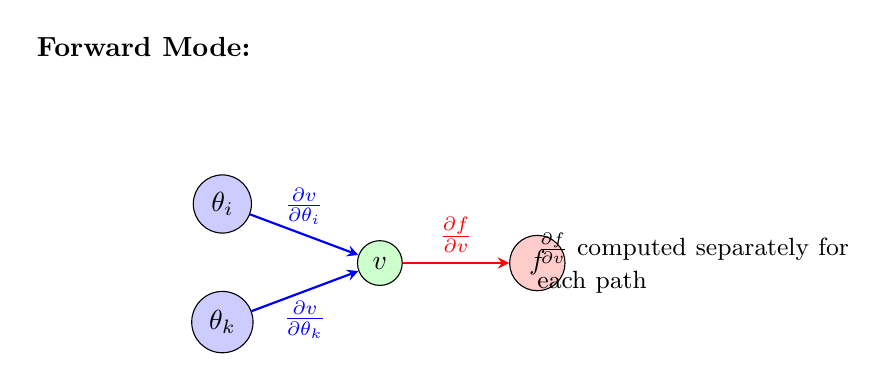
\begin{tikzpicture}[node distance=1.5cm, >=stealth]
    % Layer labels
    \node at (-1, 2) {\textbf{Forward Mode:}};
    
    % Nodes
    \node[draw, circle, fill=blue!20] (theta1) at (0, 0) {$\theta_i$};
    \node[draw, circle, fill=blue!20] (theta2) at (0, -1.5) {$\theta_k$};
    \node[draw, circle, fill=green!20] (v) at (2, -0.75) {$v$};
    \node[draw, circle, fill=red!20] (f) at (4, -0.75) {$f$};
    
    % Edges with labels
    \draw[->, thick, blue] (theta1) -- (v) node[midway, above] {$\frac{\partial v}{\partial \theta_i}$};
    \draw[->, thick, blue] (theta2) -- (v) node[midway, below] {$\frac{\partial v}{\partial \theta_k}$};
    \draw[->, thick, red] (v) -- (f) node[midway, above] {$\frac{\partial f}{\partial v}$};
    
    % Annotation
    \node[text width=4cm] at (6, -0.75) {\small $\frac{\partial f}{\partial v}$ computed separately for each path};
\end{tikzpicture}
\end{center}

\subsection{Backpropagation: The Efficient Solution}

\textbf{Key Insight:} If we compute $\frac{\partial f}{\partial v}$ for all nodes $v$ in a \textit{backward} pass, we can share these computations across all weights.

The multivariable chain rule tells us:
$$\frac{\partial f}{\partial v} = \sum_{j : w_j \text{ child of } v} \frac{\partial f}{\partial w_j} \cdot \frac{\partial w_j}{\partial v}$$

If we already have $\frac{\partial f}{\partial w_j}$ from the backward pass, we can compute $\frac{\partial f}{\partial v}$ using only \textbf{local} information.

\begin{algorithm}[Backpropagation]
\textbf{Forward Pass:}
\begin{enumerate}
    \item Compute all activations $v^{(l)}$ layer by layer
    \item Store intermediate values $(u^{(l)}, v^{(l)})$ for the backward pass
\end{enumerate}

\textbf{Backward Pass:}
\begin{enumerate}
    \item Initialize $\delta^{(L)} := \frac{\partial \mathcal{L}}{\partial v^{(L)}}$ at the output layer
    \item \textbf{for} $l = L-1$ down to $1$ \textbf{do}
    \begin{enumerate}
        \item Compute $\delta^{(l)} = (W^{(l+1)})^\top \delta^{(l+1)} \odot \sigma'(u^{(l)})$
        \item Compute $\frac{\partial \mathcal{L}}{\partial W^{(l)}} = \delta^{(l)} (v^{(l-1)})^\top$
        \item Compute $\frac{\partial \mathcal{L}}{\partial b^{(l)}} = \delta^{(l)}$
    \end{enumerate}
    \item \textbf{end for}
\end{enumerate}
\end{algorithm}

Here $\delta^{(l)} = \frac{\partial \mathcal{L}}{\partial u^{(l)}}$ is the ``error signal'' at layer $l$, and $\odot$ denotes element-wise multiplication.

\begin{theorem}[Backprop Complexity]
Backpropagation computes all partial derivatives in $O(E)$ time, where $E$ is the number of edges (weights) in the network.
\end{theorem}

\begin{proof}
Each edge is visited exactly once in the forward pass (to compute activations) and exactly once in the backward pass (to compute gradients). Each visit requires $O(1)$ operations. Therefore, total time is $O(E)$.
\end{proof}

\textbf{Comparison:}
\begin{center}
\begin{tabular}{ll}
\hline
\textbf{Method} & \textbf{Time Complexity} \\
\hline
Numerical differentiation & $O(WE)$ (finite differences) \\
Forward mode autodiff & $O(WE)$ \\
\textbf{Backpropagation} & $O(E)$ \\
\hline
\end{tabular}
\end{center}

\newpage
\section{The Vanishing and Exploding Gradient Problem}

\subsection{The Vanishing Gradient Problem}

Consider a deep network with $L$ layers and sigmoid activations. The gradient at layer $l$ involves:
$$\frac{\partial \mathcal{L}}{\partial W^{(l)}} \propto \prod_{k=l}^{L} \sigma'(u^{(k)}) \cdot W^{(k)}$$

\textbf{The Issue:} For sigmoid, $\sigma'(z) = \sigma(z)(1-\sigma(z))$.

\begin{proposition}
The sigmoid derivative satisfies $\sigma'(z) \leq \frac{1}{4}$ for all $z \in \mathbb{R}$, with equality at $z = 0$.
\end{proposition}

\begin{proof}
$\sigma'(z) = \sigma(z)(1-\sigma(z))$. Let $s = \sigma(z) \in (0,1)$. Then $\sigma'(z) = s(1-s)$.

By AM-GM: $s(1-s) \leq \left(\frac{s + (1-s)}{2}\right)^2 = \frac{1}{4}$, with equality when $s = 1/2$, i.e., $z = 0$.
\end{proof}

\begin{theorem}[Vanishing Gradients]
For a network with sigmoid activations and $L$ layers, if $\|W^{(k)}\| \leq 1$ for all $k$:
$$\left\|\frac{\partial \mathcal{L}}{\partial W^{(1)}}\right\| = O\left(\frac{1}{4^{L-1}}\right)$$
Gradients vanish exponentially with depth.
\end{theorem}

\subsection{The Exploding Gradient Problem}

Conversely, if $\|W^{(k)}\| > 4$, gradients can \textbf{explode} exponentially:
$$\left\|\frac{\partial \mathcal{L}}{\partial W^{(1)}}\right\| = O\left(\lambda^{L-1}\right) \quad \text{for } \lambda > 1$$

\subsection{Solutions}

\textbf{1. ReLU Activation:}
$$\sigma'(z) = \begin{cases} 1 & z > 0 \\ 0 & z \leq 0 \end{cases}$$
Gradients are either 0 or 1; no shrinking occurs in the active region.

\textbf{2. Careful Initialization (Xavier/He):}
\begin{itemize}
    \item \textbf{Xavier (Glorot):} $\text{Var}(w) = \frac{2}{n_{\text{in}} + n_{\text{out}}}$ (for tanh/sigmoid)
    \item \textbf{He:} $\text{Var}(w) = \frac{2}{n_{\text{in}}}$ (for ReLU)
\end{itemize}

The idea is to keep the variance of activations constant across layers.

\textbf{3. Batch Normalization:}

Normalize activations within each mini-batch to have mean 0 and variance 1:
$$\hat{z} = \frac{z - \mu_B}{\sqrt{\sigma_B^2 + \epsilon}}$$

This keeps activations in the ``active'' region of the activation function.

\textbf{4. Residual Connections (ResNets):}
$$h^{(l+1)} = h^{(l)} + F(h^{(l)})$$

Gradients can flow directly through the identity path, avoiding the vanishing gradient problem.

\needspace{0.33\textheight}
\section{Summary}

\subsection{The Progression of Ideas}

\begin{center}
\begin{tabular}{lll}
\hline
\textbf{Model} & \textbf{Key Insight} & \textbf{Limitation} \\
\hline
Perceptron & Linear separation via hyperplane & Only linearly separable data \\
SVM & Maximum margin + kernel trick & Fixed feature space \\
Neural Network & Nonlinear activation $\to$ UAT & Training is non-convex \\
Deep Networks & Depth gives expressiveness & Vanishing/exploding gradients \\
\hline
\end{tabular}
\end{center}

\subsection{Key Theorems}

\begin{enumerate}
    \item \textbf{Perceptron Convergence:} At most $1/\gamma^2$ mistakes
    \item \textbf{Perceptron Lower Bound:} $\Omega(2^{n-1})$ mistakes possible
    \item \textbf{Modified Perceptron:} $O(\log n / \sigma^2)$ mistakes with high probability
    \item \textbf{Universal Approximation:} Single hidden layer suffices for any continuous function
    \item \textbf{Backprop Efficiency:} $O(E)$ vs $O(WE)$ for forward mode
\end{enumerate}

\subsection{Practical Guidelines}

\begin{enumerate}
    \item Use ReLU (or variants) for hidden layers
    \item Use proper initialization (He for ReLU, Xavier for tanh/sigmoid)
    \item Consider batch normalization for deep networks
    \item Monitor gradient norms during training
    \item Use residual connections for very deep networks ($> 20$ layers)
\end{enumerate}

\end{document}
